\section{Shading Module}\label{shading-module}

\subsection{Shading and Sunlit Area Calculations}\label{shading-and-sunlit-area-calculations}

When assessing heat gains in buildings due to solar radiation, it is necessary to know how much of each part of the building is shaded and how much is in direct sunlight. As an example, the figure below shows a flat roofed, L-shaped structure with a window in each of the visible sides. The sun is to the right so that walls 1 and 3 and windows a and c are completely shaded, and wall 4 and window d are completely sunlit. Wall 2 and window b are partially shaded. The sunlit area of each surface changes as the position of the sun changes during the day. The purpose of the EnergyPlus shadow algorithm is to compute these \textbf{sunlit areas}.~ Predecessors to the EnergyPlus shadowing concepts include the BLAST and TARP shadowing algorithms.

The shadow algorithm is based on coordinate transformation methods similar to Groth and Lokmanhekim and the shadow overlap method of Walton.

Using the \textbf{ShadowCalculation} object, you can set how often the shadowing calculations are performed. Calculating them every timestep (TimestepFrequency options) is obviously the most accurate but is also be the most time consuming.~ Using a greater length of time (number of days) before calculating again can yield speedier results.~ For lengths of time greater than one day, the solar position values (e.g.~equation of time, sun position angles) are averaged over that time period for the shadowing calculations. For dynamic shading, TimestepFrequency is required to capture changes in shading transmittance.

\begin{figure}[hbtp] % fig 38
\centering
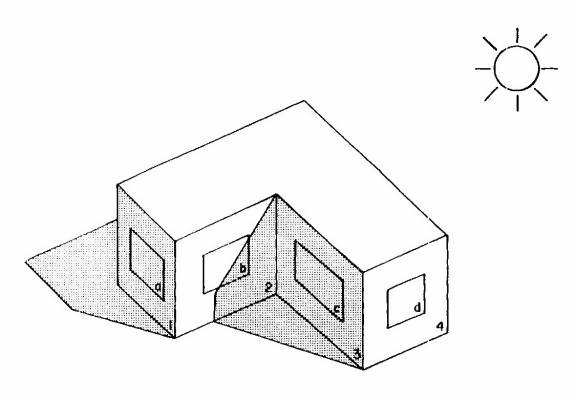
\includegraphics[width=0.9\textwidth, height=0.9\textheight, keepaspectratio=true]{media/image601.png}
\caption{Overall Shadowing Scheme Depiction \protect \label{fig:overall-shadowing-scheme-depiction}}
\end{figure}

\subsection{Solar Position}\label{solar-position}

Current solar position is described in terms of three direction cosines that are convenient for determining the angle of incidence of the sun's rays on a building surface.~ The following procedure is used to determine the direction cosines.~ The values of the solar declination angle, $\delta$, and the equation of time, $\varepsilon$, are based on \emph{Astronomical Algorithms}, Meeus.~ Solar declination is a function of local/site latitude.

The fractional year is calculated, in radians:

\begin{equation}
\gamma  = \frac{{2\pi }}{{366}}(day~of~year)
\end{equation}

From this fractional year, the equation of time and solar declination angle are calculated.~ For each time step (time value = fractional hour), the hour angle is calculated from:

\begin{equation}
HourAngle = \left( {15\cdot \left( {12 - \left( {TimeValue + EquationOfTime} \right)} \right) + \left( {TimeZoneMeridian - Longitude} \right)} \right)
\end{equation}

TimeZoneMeridian is the standard meridian for the location's time zone \{GMT +/-\}.

Solar HourAngle (\emph{H}) gives the apparent solar time for the current time period (degrees); HourAngle is positive before noon, negative after noon.~ It is common astronomical practice to express the hour angle in hours, minutes and seconds of time rather than in degrees.~ You can convert the hour angle displayed from EnergyPlus to time by dividing by 15.~ (Note that 1 hour is equivalent to 15 degrees; 360° of the Earth's rotation takes place every 24 hours.)~ The relationship of angles in degrees to time is shown in the following table:

% table 23
\begin{longtable}[c]{@{}ll@{}}
\caption{Relationship of Angles (degrees) to Time \label{table:relationship-of-angles-degrees-to-time}} \tabularnewline
\toprule 
Unit of Angle & Equivalent time \tabularnewline
\midrule
\endfirsthead

\caption[]{Relationship of Angles (degrees) to Time} \tabularnewline
\toprule 
Unit of Angle & Equivalent time \tabularnewline
\midrule
\endhead

1 radian & 3.819719 hours \tabularnewline
1 degree & 4 minutes \tabularnewline
1 arcmin & 4 seconds \tabularnewline
1 arcsec & 0.066667 seconds \tabularnewline
\bottomrule
\end{longtable}

The Solar Altitude Angle ($\beta$) is the angle of the sun above the horizontal (degrees). The Solar Azimuth Angle ($\phi$) is measured from the North (clockwise) and is expressed in degrees.~ This is shown more clearly in the following figure.

\begin{figure}[hbtp] % fig 39
\centering
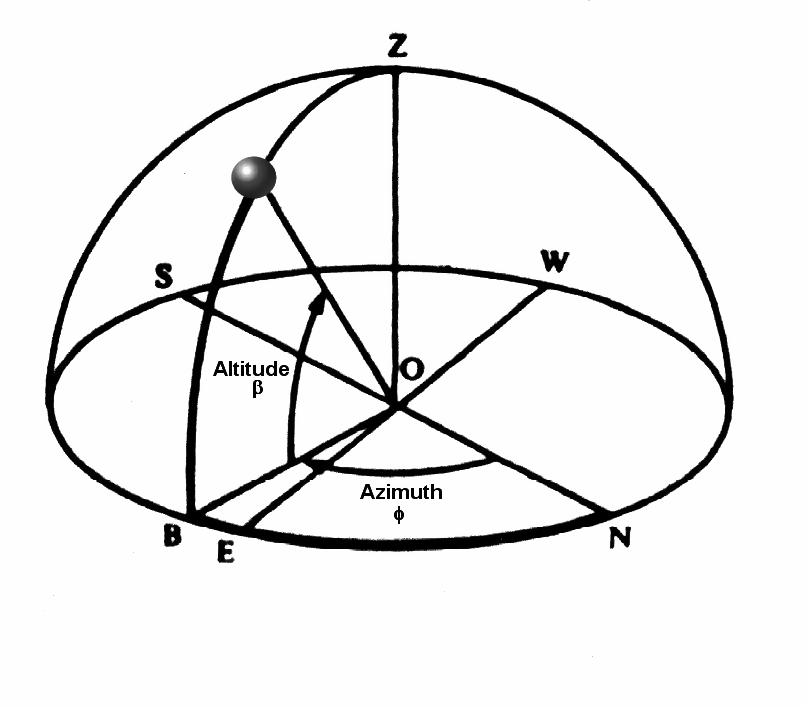
\includegraphics[width=0.9\textwidth, height=0.9\textheight, keepaspectratio=true]{media/image604.png}
\caption{Solar Position Illustration \protect \label{fig:solar-position-illustration}}
\end{figure}

\subsection{Surface Geometry}\label{surface-geometry}

Shadow calculations first require that the building surfaces be described geometrically. Surfaces are described by the coordinates of their vertices in a three dimensional Cartesian coordinate system. This Right-hand coordinate system has the X-axis pointing east, the Y-axis pointing north, and the Z-axis pointing up (see figure below). The azimuth angle ($\psi$) of a surface is the angle from the north axis to the projection onto the X-Y plane of a normal to the surface (clockwise positive). The surface tilt angle ($\phi$) is the angle between the Z-axis and the normal to the surface. The vertices are recorded in counter-clockwise sequence (as the surface is viewed from outside its zone).

During surface entry, surfaces are checked for convex or non-convex shape. If non-convex and inappropriate (used as a receiving surface) then a severe error is produced telling the user that shadowing calculations may be inaccurate.

Similarly collinear points (or as noted below, points within 1 mm distance) are removed unless removing would make an illegal surface (less than 3 points). But degenerate collinear surfaces \emph{should} be removed -- they make the shadowing routines do extra work which takes extra time.

Collinear -- points that essentially form a ``line'' rather than a surface shape.

Resolution of 1mm or less -- near collinear points.

Note that the resolution on surfaces/shadowing is 1 mm -- using resolution beyond that will result in truncation of the shadowing.

\begin{figure}[hbtp] % fig 40
\centering
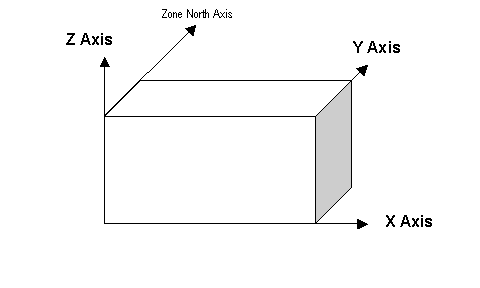
\includegraphics[width=0.9\textwidth, height=0.9\textheight, keepaspectratio=true]{media/image605.png}
\caption{EnergyPlus Coordinate System \protect \label{fig:energyplus-coordinate-system}}
\end{figure}

The GlobalGeometryRules object specifies to EnergyPlus how the surface vertices will be presented in the input file.~ Of pertinent interest here is that the user may specify the vertices in either ``relative'' or ``world'' coordinates.~ Regardless of input specifications, when vertices are reported, they are reported in world coordinates, starting at the upper-left-corner (4-sided surface) and are listed counter-clockwise.

\subsubsection{Relative Coordinate Transformation}\label{relative-coordinate-transformation}

When vertices are specified in ``relative'' coordinates, there can be a ``building'' north axis as well as a ``zone'' north axis.~ The building north axis/coordinate system is a rotation of $\psi_b$ degrees from the global/world coordinate system.~ The global coordinates of zone origins are related to the building relative coordinates by:

\begin{equation}
{X_{zo}} = {X_{br}}\cdot \cos {\psi_b} - {Y_{br}}\cdot \sin {\psi_b}
\end{equation}

\begin{equation}
{Y_{zo}} = {Y_{br}}\cdot \sin {\psi_b} - {Y_{br}}\cdot \cos {\psi_b}
\end{equation}

\begin{equation}
{Z_{zo}} = {Z_{br}}
\end{equation}

Where

zo -- represents Zone Origin

br -- represents the Zone Origin as input (relative to building origin)

The zone may also be rotated $\psi$\(_{z}\) degrees relative to the building coordinates. Origins of zone surfaces are then given relative to the zone coordinate system. The global coordinates of the surface origins are calculated by:

\begin{equation}
{X_{so}} = {X_{zo}} + {X_{zr}}\cdot \cos {\psi_z} - {Y_{zr}}\cdot \sin {\psi_z}
\end{equation}

\begin{equation}
{Y_{so}} = {Y_{zo}} + {X_{zr}}\cdot \sin {\psi_z} - {Y_{zr}}\cdot \cos {\psi_z}
\end{equation}

\begin{equation}
{X_{so}} = {X_{zo}} + {X_{zr}}\cdot \cos {\psi_z} - {Y_{zr}}\cdot \sin {\psi_z}
\end{equation}

A surface azimuth angle relative to the zone coordinate system ($\psi$\(_{s}\)) is converted to a global azimuth by:

\begin{equation}
\psi  = {\psi_s} + {\psi_z} + {\psi_b}
\end{equation}

The surface tilt angle ($\phi$) is not changed by these rotations about the Z-axis.

The coordinates of the surface vertices are given in a coordinate system in the plane of the surface relative to the second vertex as shown for surfaces in Figure~\ref{fig:energyplus-coordinate-system}. The X-axis of the surface coordinate system is a horizontal line through the second vertex. The global coordinates of the surface vertices are given by:

\begin{equation}
X = {X_{so}} + {X_{sr}}\cdot \cos \psi  - {Y_{sr}}\cdot \sin \psi \cdot \cos \phi
\end{equation}

\begin{equation}
Y = {Y_{so}} + {X_{sr}}\cdot \sin \psi  - {Y_{sr}}\cdot \cos \psi \cdot \cos \phi
\end{equation}

\begin{equation}
Z = {Z_{so}} + {Y_{sr}}\cdot \sin \phi
\end{equation}

\subsubsection{World Coordinates to Relative Coordinates}\label{world-coordinates-to-relative-coordinates}

Vertices in the global coordinate system can be transformed to the coordinate system relative to a given surface by

\begin{equation}
{X'} = X - {X_{so}}
\end{equation}

\begin{equation}
{Y'} = Y - {Y_{so}}
\end{equation}

\begin{equation}
{Z'} = Z - {Z_{so}}
\end{equation}

\begin{equation}
{X_{sr}} =  - {X'}\cdot \cos \psi  + {Y'}\cdot \sin \psi
\end{equation}

\begin{equation}
{Y_{sr}} =  - {X'}\cdot \sin \psi \cdot \cos \phi  + {Y'}\cdot \cos \psi \cdot \cos \phi  + {Z'}\cdot \sin \phi
\end{equation}

\begin{equation}
{Z_{sr}} =  - {X'}\cdot \sin \psi \cdot \sin \phi  + {Y'}\cdot \cos \psi \cdot \sin \phi  + {Z'}\cdot \cos \phi
\label{eq:ZsrEquation}
\end{equation}

\subsection{Shadow Projection}\label{shadow-projection}

All architectural forms are represented by plane polygons. This can give good accuracy even for curved surfaces: a sphere can be approximated by the 20 nodes of an icosahedron with only 3 percent error in the shadow area cast by the sphere. Consider how a solid object, which is composed of a set of enclosing plane polygons, casts a shadow. Figure~\ref{fig:basic-shadowing-concept-structure} shows a box shaped structure on a horizontal surface. The structure consists of a top (surface 1) and four vertical surfaces (2 and 3 visible to the observer and 4 and 5 not visible). The sun is positioned behind and to the right of the structure and a shadow is cast onto the horizontal surface (the ground).

Surfaces 1, 4, and 5 are in sunlight; 2 and 3 are in shade. It is possible to think of the structure's shadow as the combination of shadows cast by surfaces 1, 2, 3, 4 and 5 or by 1, 4 and 5, or by surfaces 2 and 3.~ This last combination of shadow casting surfaces is the simplest. In the EnergyPlus shadow algorithm every surface is considered to be one of the surfaces that enclose a solid, and only those surfaces that are not sunlit at a given hour are considered shadowing surfaces.

\begin{figure}[hbtp] % fig 41
\centering
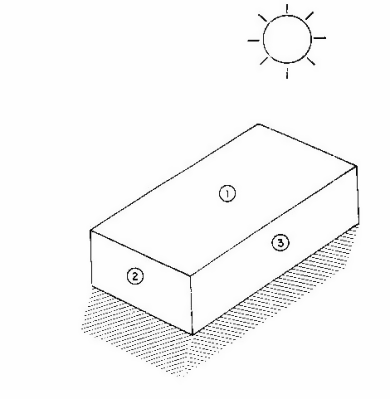
\includegraphics[width=0.9\textwidth, height=0.9\textheight, keepaspectratio=true]{media/image622.png}
\caption{Basic shadowing concept structure \protect \label{fig:basic-shadowing-concept-structure}}
\end{figure}

The expressions in Equation~\ref{eq:ZsrEquation} are the direction cosines of the surface:

\begin{equation}
C{W_1} = \sin \psi \cdot \cos \phi
\end{equation}

\begin{equation}
C{W_2} = \cos \psi \cdot \sin \phi
\end{equation}

\begin{equation}
C{W_3} = \cos \phi
\end{equation}

The cosine of the angle of incidence of the sun's rays on the surface are given by the dot product of surface and sun direction cosines.

\begin{equation}
\cos \theta  = C{S_1}\cdot C{W_1} + C{S_2}\cdot C{W_2} + C{S_3}\cdot C{W_3}
\end{equation}

If \(\cos \theta\) ~is less than zero, the sun is behind the surface.

A shadow is projected from the vertices of the shadowing polygon (SP) along the direction of the sun's rays to the plane of the shadow receiving polygon (RP).~ If any vertices of the SP are below the plane of the RP (z \textless{} 0), a false shadow is cast as in Figure~\ref{fig:illustration-of-shadow-clipping}.~ The ``submerged'' portion of the SP must be clipped off before projection.

\begin{figure}[hbtp] % fig 42
\centering
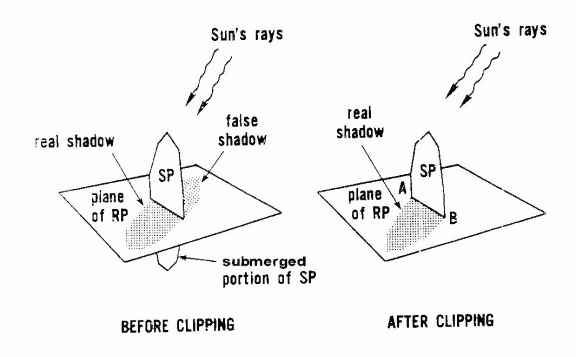
\includegraphics[width=0.9\textwidth, height=0.9\textheight, keepaspectratio=true]{media/image628.png}
\caption{Illustration of Shadow Clipping \protect \label{fig:illustration-of-shadow-clipping}}
\end{figure}

This is done by finding, through linear interpolation, the points on the perimeter of the SP, which intersect the plane of the RP. These points become new vertices of the SP, which together with the other positive vertices define a clipped SP that casts only a real shadow.

A vertex located at (x, y, z) relative to the RP coordinate system casts a shadow to a point in the plane of the RP given by

\begin{equation}
{x'} = x - \frac{{z\cdot a}}{{\cos \theta }}
\end{equation}

\begin{equation}
{y'} = y - \frac{{z\cdot b}}{{\cos \theta }}
\end{equation}

where

\begin{equation}
a = \sin \psi \cdot C{S_1} - \cos \psi \cdot C{S_2}
\end{equation}

and

\begin{equation}
b =  - \cos \psi \cdot \cos \phi \cdot C{S_1} - \sin \psi \cdot \cos \phi \cdot C{S_2} + \sin \phi \cdot C{S_3}
\end{equation}

More explicitly, a casting surface -- a shadow casting surface or general casting surface -- is one that casts a shadow on other surfaces. A receiving surface -- a shadow receiving surface -- is one that receives shadows from other surfaces (i.e.~casting surfaces). A back surface -- an inside surface -- is one that may be partially sunlit/receive solar transmission for interior solar distribution.

\subsection{Homogeneous Coordinates}\label{homogeneous-coordinates}

Two-dimensional homogeneous coordinate techniques are used to determine the vertices of shadow overlaps. In homogeneous coordinates, points and lines are represented by a single form that allows simple vector operations between those forms {[}Newman-Sproul{]}.~ A point (X, Y) is represented by a three element vector (x, y, w) where x = w*X, y = w*Y, and w is any real number except zero. A line is also represented by a three element vector (a, b, c). The directed line (a, b, c) from point (x\(_{1}\), y\(_{1}\), w\(_{1}\)) to point (x\(_{2}\), y\(_{2}\), w\(_{2}\)) is given by:

\begin{equation}
(a,b,c) = ({x_1},{y_1},{z_1}) \otimes ({x_2},{y_2},{z_2})
\end{equation}

The sequence in the cross product is a convention to determine sign. The condition that a point (x, y, w) lie on a line (a, b, c) is that

\begin{equation}
(a,b,c) \bullet (x,y,w) = 0
\end{equation}

The point is normalized by dividing by w. Then if

\begin{equation}
(a,b,c) \bullet (x/w,y/w,1) > 0
\end{equation}

the point is to the left of the line.~ If it is less than zero, the point is to the right of the line. The intercept (x, y, w) of line (a\(_{1}\), b\(_{1}\), c\(_{1}\)) and line (a\(_{2}\), b\(_{2}\), c\(_{2}\)) is given by:

\begin{equation}
(x,y,w) = ({a_1},{b_1},{c_1}) \otimes ({a_2},{b_2},{c_2})
\end{equation}

Note that the use of homogeneous coordinates as outlined above provides a consistent method and notation for defining points and lines, for determining intercepts, and for determining whether a point lies to the left, to the right, or on a line.~ Normalization provides the means for transforming to and from homogeneous notation and Cartesian coordinates.~ Thus, if (X, Y) is a Cartesian coordinate pair, its homogeneous coordinates are (X, Y, 1).~ Similarly, the homogeneous coordinates (x, y, w) can be transformed to the Cartesian point with coordinates (x/w, y/w).

\subsection{Polygon Clipping Algorithms}\label{polygon-clipping-algorithms}

Two methods for polygon clipping (treating of overlapping shadows) are currently in use in EnergyPlus.

\begin{itemize}
\item
  Convex Weiler - Atherton
\item
  Sutherland -- Hodgman
\end{itemize}

The original EnergyPlus method for polygon clipping is a special version of the Weiler-Atherton model (Weiler, Atherton, 1977). It was developed to be sufficiently general to clip concave polygons with holes. The implementation in the current version of EnergyPlus, however, does not support concave shadowing surfaces or holes. The relative computational complexity is preserved -- the algorithm is carried out in four steps. For example, if A and B are polygons (see Figure~\ref{fig:point-a-vertex-of-a-enclosed-by-b}).

1)~~~A call to INCLOS determines which vertices of X lie within Y.

2)~~~A second call determines which vertices of Y lie within X.

3)~~~If neither polygon is contained completely within the other, INTCPT is called to collect points of intersection between X and Y.

4)~~~Since the points are usually gathered out of order, they must then be oriented.

The Sutherland-Hodgman algorithm (Sutherland, Hodgman, 1974) is less complex compared to the Weiler-Atherton method and is well-suited to clipping convex polygons. In actuality, only convex shading surfaces are currently supported by EnergyPlus. Let X be a polygon called the ``subject polygon'' (SP) and Y be a polygon called the ``clipping polygon'' (CP). The method performs the computation by iterating over the edges of the CP and removing points from the SP that fall in the clipping plane, i.e.~points that fall to the left of the edge of the CP. Intersections between the clip edge and the edges of the SP are added appropriately, and points falling outside of the clipping plane, i.e.~to the right of the edge of the CP, are added the output polygon as well. This resultant polygon is stored and the process is repeated for the rest of the clip edges in CP. The process is analogous to cutting off pieces of the SP one-by-one with respect to each edge of the CP. The result is ordered and identical to the polygon produced by the Weiler-Atherton method.

\subsection{Overlapping Shadows}\label{overlapping-shadows}

After transforming the shadows onto the plane of the receiving surface, the basic job of the shadow algorithm is to determine the area of the overlap between the polygons representing the shadows and the polygon representing the receiving surface. Concave surfaces are supported only for exterior wall heat transfer surfaces, when using SutherlandHodgman option. Concave shading devices are not supported by the this option. Neither concave shading devices nor concave exterior wall heat transfer surfaces are supported by the ConvexWeilerAtherton clipping routine.

When only convex shading devices are considered, this provides a great simplification. The overlap between two convex polygons (i.e.~projections of shading devices via the direction of the sun) is another convex polygon. Coordinate and projection transformations of a convex polygon produce another convex polygon. Any non-convex polygon can be constructed as the union of convex ones.

For ConvexWeilerAtherton, there is considerable simplification if only convex (no interior angle \textgreater{} 180 ) polygons are considered. The overlap between two convex polygons is another convex polygon. Coordinate and projection transformations of a convex polygon produce another convex polygon. Any non-convex polygon can be constructed as a sum of convex ones.

The vertices that define the overlap between two convex polygons, A and B, consist of:

\begin{itemize}
\item
  the vertices of A enclosed by B
\item
  the vertices of B enclosed by A
\item
  and the intercepts of the sides of A with the sides of B
\end{itemize}

In Figure~\ref{fig:point-a-vertex-of-a-enclosed-by-b}, point a is the result of rule 1, point c is the result of rule 2, and points b and d result from rule 3. The overlap of A and B is the polygon a-b-c-d. Figure~\ref{fig:surface-a-totally-overlaps-surface-b.} shows an overlap where all of the vertices of B are enclosed by A.~ Figure~\ref{fig:figure-formed-from-intercept-overlaps-between} shows an overlap defined only by the intercepts of A and B. Figure~\ref{fig:complex-overlapping-condition} shows a more complex overlap.

\begin{figure}[hbtp] % fig 43
\centering
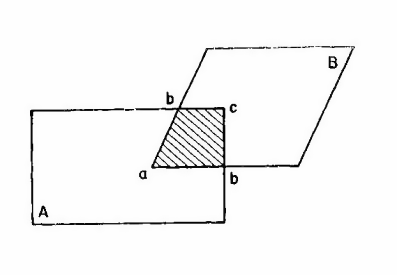
\includegraphics[width=0.9\textwidth, height=0.9\textheight, keepaspectratio=true]{media/image637.png}
\caption{Point a – Vertex of A Enclosed by B \protect \label{fig:point-a-vertex-of-a-enclosed-by-b}}
\end{figure}

Coordinate transformation retains the order of the vertices of a polygon, while a projection reverses the order. The sequence of vertices of the receiving polygons should be reversed so it and all shadow polygons will have the same sequence.

\begin{figure}[hbtp] % fig 44
\centering
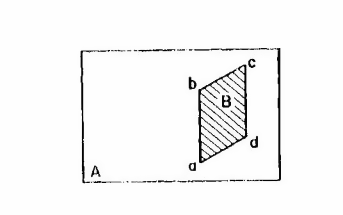
\includegraphics[width=0.9\textwidth, height=0.9\textheight, keepaspectratio=true]{media/image638.png}
\caption{Surface A Totally Overlaps Surface B. \protect \label{fig:surface-a-totally-overlaps-surface-b.}}
\end{figure}

A point is enclosed by a clockwise, convex polygon if the point lies to the right of all sides (or does not lie to the left of any side) of the polygon.~ The intercept of two sides may not lie beyond the ends of either side. These are ``line segments'' rather than ``lines''. It is possible to tell if line segments A and B intercept within their end points by noting that the ends of A must lie on both sides of B, and the ends of B must lie on both sides of A. This should be done before the intercept is calculated.

\begin{figure}[hbtp] % fig 45
\centering

\includegraphics[width=0.9\textwidth, height=0.9\textheight, keepaspectratio=true]{media/image639.png}
\caption{Figure Formed from Intercept Overlaps Between A and B \protect \label{fig:figure-formed-from-intercept-overlaps-between}}
\end{figure}

Once the vertices are determined, they must be sorted into clockwise order for the area to be computed.~ Given a closed, planar polygon of n sequential vertices (x\(_{1}\), y\(_{1}\)), (x\(_{2}\), y\(_{2}\)), \ldots{}, (x\(_{n}\), y\(_{n}\)), its \textbf{area} is given:

\begin{equation}
Area = {\frac{1}{2}}\sum\limits_{i = 1}^n {({x_i}{y_{i + 1}} - {x_{i + 1}}{y_i})}
\end{equation}

where (x\(_{n+1}\),y\(_{n+1}\)) = (x\(_{1}\), y\(_{1}\))

The area is positive if the vertices are counter-clockwise and negative if they are clockwise.

\begin{figure}[hbtp] % fig 46
\centering

\includegraphics[width=0.9\textwidth, height=0.9\textheight, keepaspectratio=true]{media/image641.png}
\caption{Complex Overlapping Condition \protect \label{fig:complex-overlapping-condition}}
\end{figure}

If two shadows overlap the receiving surface, they may also overlap each other as in Figure~\ref{fig:multiple-shadow-overlaps}. The vertices of this overlap can be computed.~ The areas of all overlaps can be computed.~ The total sunlit area can be expressed as the sum of all polygon areas given a proper sign on each of the areas.

The following convention was adopted:

% table 24
\begin{longtable}[c]{@{}ll@{}}
\caption{Surface / Area Characteristic / Convention \label{table:surface-area-characteristic-convention}} \tabularnewline
\toprule 
Surface Characteristic & Area Convention \tabularnewline
\midrule
\endfirsthead

\caption[]{Surface / Area Characteristic / Convention} \tabularnewline
\toprule 
Surface Characteristic & Area Convention \tabularnewline
\midrule
\endhead

receiving surface & positive (A) \tabularnewline
overlap between shadow and receiving & negative (B  \&  C) \tabularnewline
overlap between two shadows & positive (D) \tabularnewline
\bottomrule
\end{longtable}

and so on through multiple overlaps where the sign of the overlap area is the product of the signs of the overlapping areas.

\begin{figure}[hbtp] % fig 47
\centering

\includegraphics[width=0.9\textwidth, height=0.9\textheight, keepaspectratio=true]{media/image642.png}
\caption{Multiple Shadow Overlaps \protect \label{fig:multiple-shadow-overlaps}}
\end{figure}

Partially transparent shadowing surfaces can also be modeled by giving a transparency ($\tau$) to every shadowing polygon. Let $\tau$ of the receiving polygon be one. Then the $\tau$ of every overlap of polygons i and j is the product of $\tau$\(_{i}\)and $\tau$\(_{j}\). The shaded area is then computed by summing A\(_{i}\)*(1 - $\tau$\(_{i}\)) for all overlap polygons.

It is easy to determine the sunlit area of a window once all the shadow and overlap vertices on the wall have been computed. Consider wall 2 of Figure~\ref{fig:overall-shadowing-scheme-depiction}. First, the wall is considered a simple rectangle and the window on it is ignored. The shadow overlapping is performed and the sunlit portion of the gross wall area is computed. Then the window rectangle is overlapped with the shadow to determine its sunlit area. The sunlit area of the window is subtracted from the gross wall sunlit area to determine the net wall sunlit area. During this calculation it is not necessary to recompute the shadows, because they were precisely determined on the wall.

When the SutherlandHodgman option is selected, the overlap is computed using the Sutherland-Hodgman algorithm for polygon clipping when. Let X be a polygon called the ``subject polygon'' (SP) and Y be a polygon called the ``clipping polygon'' (CP). The method performs the computation by iterating over the edges of the CP and removing points from the SP that fall in the clipping plane, i.e.~points that fall to the left of the edge of the CP. If it is to the left of any edge, it the point does not overlap with the CP. Intersections between the clip edge and the edges of the SP are added appropriately, and points falling outside of the clipping plane, i.e.~to the right of the edge of the CP, are added the output polygon as well. This resultant polygon is stored and the process is repeated for the rest of the clip edges in CP. The process is analogous to cutting off pieces of the SP one-by-one with respect to each edge of the CP. Note that the SP may be concave, but the CP may not. This means that the exterior wall surfaces may be concave, while shading devices may not be concave.

\subsection{Solar Gains}\label{solar-gains-000}

The total solar gain on any exterior surface is a combination of the absorption of direct and diffuse solar radiation given by

\begin{equation}
{Q_{so}} = \alpha \cdot \left( {{I_b}\cdot \cos \theta \cdot \frac{{{S_s}}}{S} + {I_s}\cdot {F_{ss}} + {I_g}\cdot {F_{sg}}} \right)
\end{equation}

where

$\alpha$ = solar absorptance of the surface

A = angle of incidence of the sun's rays

S = area of the surface

S\(_{s}\) = sunlit area

I\(_{b}\) = intensity of beam (direct) radiation

I\(_{s}\) = intensity of sky diffuse radiation

I\(_{g}\) = intensity of ground reflected diffuse radiation

F\(_{ss}\) = angle factor between the surface and the sky

F\(_{sg}\) = angle factor between the surface and the ground

For the surface of a building located on a featureless plain

\begin{equation}
{F_{ss}} = \frac{{1 + \cos \phi }}{2}
\end{equation}

and

\begin{equation}
{F_{sg}} = \frac{{1 - \cos \phi }}{2}
\end{equation}

If the surface is shaded the program modifies \emph{F\(_{ss}\)} by a correction factor that takes into account the radiance distribution of the sky (see ``Shadowing of Sky Diffuse Solar Radiation'').

Shading of ground diffuse solar radiation is not calculated by the program. It is up to the user to estimate the effect of this shading and modify the input value of \emph{F\(_{sg}\)} accordingly.

\subsection{Solar Distribution}\label{solar-distribution}

As discussed in the Input Output Reference (Object: Building), the field Solar Distribution, in the ``Building'' input object, determines how EnergyPlus will treat beam solar radiation entering a zone through exterior windows.~ There are five choices: \textbf{MinimalShadowing}, \textbf{FullExterior}, \textbf{FullInteriorAndExterior, FullExteriorWithReflections}, and \textbf{FullInteriorAndExteriorWithReflections}.

\subsubsection{MinimalShadowing}\label{minimalshadowing}

In this case, there is no exterior shadowing except from window and door reveals. All beam solar radiation entering the zone is assumed to fall on the floor, where it is absorbed according to the floor's solar absorptance. Any reflected by the floor is added to the transmitted diffuse radiation, which is assumed to be uniformly distributed on all interior surfaces. If no floor is present in the zone, the incident beam solar radiation is absorbed on all interior surfaces according to their absorptances. The zone heat balance is then applied at each surface and on the zone's air with the absorbed radiation being treated as a flux on the surface.

\subsubsection{FullExterior}\label{fullexterior}

In this case, shadow patterns on exterior surfaces caused by detached shading, wings, overhangs, and exterior surfaces of all zones are computed. As for MinimalShadowing, shadowing by window and door reveals is also calculated. Beam solar radiation entering the zone is treated as for MinimalShadowing.

\subsubsection{FullExteriorWithReflections}\label{fullexteriorwithreflections}

This case is the same interior distribution as the preceding option but uses exterior reflections as well (see the section Solar Radiation Reflected from Exterior Surfaces for further explanation).

\subsubsection{FullInteriorAndExterior}\label{fullinteriorandexterior}

This is the same as FullExterior except that instead of assuming all transmitted beam solar falls on the floor the program calculates the amount of beam radiation falling on each surface in the zone, including floor, walls and windows, by projecting the sun's rays through the exterior windows, taking into account the effect of exterior shadowing surfaces and window shading devices.

If this option is used, you should be sure that the surfaces of the zone totally enclose a space. This can be determined by viewing the \textbf{eplusout.dxf} file with a program like AutoDesk's Volo View Express. You should also be sure that the zone is \textbf{convex}. Examples of convex and non-convex zones are shown in Figure~\ref{fig:illustration-of-convex-and-non-convex-zones}. The most common non-convex zone is an L-shaped zone. (A formal definition of convex is that any straight line passing through the zone intercepts at most two surfaces.)~ If the zone's surfaces do not enclose a space or if the zone is not convex you should use Solar Distribution = \textbf{FullExterior} instead of \textbf{FullInteriorAndExterior}.

If you use \textbf{FullInteriorAndExterior} the program will calculate how much beam radiation falling on an interior window is absorbed by the window, how much is reflected back into the zone, and how much is transmitted into the adjacent zone. (Interior windows are assumed to have no shading device).

If you use \textbf{FullInteriorAndExterior} the program will also calculate how much beam radiation falling on the inside of an exterior window (from other windows in the zone) is absorbed by the window, how much is reflected back into the zone, and how much is transmitted to the outside. In this calculation the effect of an interior or exterior shading device, if present, is accounted for.

\subsubsection{FulInteriorAndlExteriorWithReflections}\label{fulinteriorandlexteriorwithreflections}

This case is the same interior distribution as the preceding option but uses exterior reflections as well (see Solar Radiation Reflected from Exterior Surfaces for further explanation).

\begin{figure}[hbtp] % fig 48
\centering
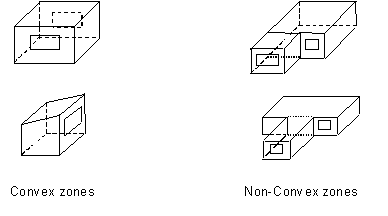
\includegraphics[width=0.9\textwidth, height=0.9\textheight, keepaspectratio=true]{media/image646.png}
\caption{Illustration of Convex and Non-convex Zones \protect \label{fig:illustration-of-convex-and-non-convex-zones}}
\end{figure}

\subsection{Details of the Interior Solar Distribution Calculation}\label{details-of-the-interior-solar-distribution-calculation}

EnergyPlus calculates the distribution of short-wave radiation in the interior of each thermal zone. This radiation consists of beam solar radiation, diffuse solar radiation, and short-wave radiation from electric lights. The program determines the amount of this radiation that is (1) absorbed on the inside face of opaque surfaces, (2) absorbed in the glass and shading device layers of the zone's exterior and interior windows, (3) transmitted through the zone's interior windows to adjacent zones, and (4) transmitted back out of the exterior windows. The effects of movable shading devices on the exterior windows are taken into account; \emph{the program does not allow shading devices on interior windows}. Most of this calculation is done in subroutine CalcInteriorSolarDistribution in the SolarShading module.

\subsubsection{Initial Distribution of Diffuse Solar Transmitted through Exterior and Interior Windows}\label{initial-distribution-of-diffuse-solar-transmitted-through-exterior-and-interior-windows}

Diffuse solar (from sky and ground sources) transmitted through exterior windows is first distributed to the interior heat transfer surfaces in the zone containing the exterior windows. This initial distribution apportions the transmitted diffuse solar to interior surfaces using the approximate view factors described above in ``LW Radiation Exchange Among Zone Surfaces.'' The amount of this initially distributed diffuse solar absorbed by each interior surface, and each window material layer, is calculated and later added to the ``short-wave radiation absorbed'' values described below. The amount of this initially distributed diffuse solar that is reflected is accumulated for each zone and redistributed uniformly as part of the QD calculation described below. The amount of this initially distributed diffuse solar that is transmitted by interior windows to adjacent zones is initially distributed to the interior heat transfer surfaces in the adjacent zone in the same manner as just described.

This new treatment of diffuse solar is intended to more accurately account for the initial absorption, transmittance, and reflection of short-wave radiation prior to the uniform distribution described below.

\subsubsection{Interior Solar Radiation Absorbed by Opaque Surfaces}\label{interior-solar-radiation-absorbed-by-opaque-surfaces}

The short-wave radiation absorbed on the inside face of an opaque surface (floor, wall or ceiling) is given by:

\begin{equation}
\begin{array}{l}
QRadSWInAbs(SurfNum) = QS(ZoneNum)*AbsIntSurf(SurfNum) \\
\quad \quad \quad \quad+ AISurf(SurfNum)*BeamSolarRad [W/m^2]
\end{array}
\label{eq:ShortWaveRadInsideFaceOpaqueSurf}
\end{equation}

where

\emph{SurfNum} = surface number

\emph{ZoneNum =}number of zone that surface belongs to

\emph{QS(ZoneNum)} = short-wave diffuse irradiance in the zone {[}W/m\(^{2}\){]}

\emph{AbsIntSurf(SurfNum)} = inside solar absorptance of the surface

\emph{AISurf(SurfNum)} = inside beam solar irradiance factor for the surface {[}-{]}

\emph{BeamSolarRad} = outside beam normal solar irradiance {[}W/m\(^{2}\){]}

\paragraph{Interior Diffuse Radiation}\label{interior-diffuse-radiation}

\emph{QS} is assumed to be uniformly distributed throughout the zone. It is calculated as follows. Let \emph{Q\(_{sw}\)} be the total diffuse short-wave radiation entering the zone or originating in the zone. Since \emph{Q\(_{sw}\)} is ultimately absorbed or transmitted by zone heat transfer surfaces, summing over these surfaces gives the following energy balance equation:

\begin{equation}
\sum\limits_{i = 1}^{{N_{surf}}} {QS(ZoneNum)*{\alpha_i}{A_i} = {Q_{SW}}(ZoneNum)}
\end{equation}

where

\emph{i} = zone surface number counter

\emph{N\(_{surf}\)} = number of heat transfer surfaces in zone

\emph{A\(_{i}\)} = surface area {[}m\(^{2}\){]}

\({\alpha_i}\) = inside solar absorptance for an opaque surface, or, for a window, $\alpha_i$ = back diffuse transmittance plus back diffuse system absorptance of glass layers and shading device layers (if present)

Solving this equation for \emph{QS} gives:

\begin{equation}
QS(ZoneNum) = \frac{{{Q_{SW}}(ZoneNum)}}{{\sum\limits_{i = 1}^{{N_{surf}}} {AbsInsSur{f_i}{A_i}} }} = {Q_{SW}}(ZoneNum)*VMULT(ZoneNum)
\end{equation}

where

\begin{equation}
VMULT(ZoneNum) = \frac{1}{{\sum\limits_{i = 1}^{{N_{surf}}} {AbsIntSur{f_i}*{A_i}} }}{\rm{    [}}{{\rm{m}}^{{\rm{ - 2}}}}]
\end{equation}

and \emph{Q\(_{sw}\)} is given by:

\begin{equation}
\begin{array}{l}
{Q_{SW}} = QD(ZoneNum) + ZoneIntGain(ZoneNum)\% QLTSW \\
\quad \quad \quad + ZoneIntGain(ZoneNum)\% T\_QLTSW [W]
\end{array}
\end{equation}

where

\emph{ZoneIntGain(ZoneNum)\%QLTSW} = short-wave radiation into zone from general (overhead) electric lighting {[}W{]}

\emph{ZoneIntGain(}ZoneNum\emph{)\%T\_QLTSW} = short-wave radiation into zone from task electric lighting {[}W{]}

\emph{QD(ZoneNum)} = diffuse solar radiation entering or originating in zone {[}W{]}

\emph{QD(ZoneNum)} is given by:

\begin{equation}
\begin{array}{l}
QD(ZoneNum) = DBZone(ZoneNum)*BeamSolarRad \\
\quad \quad \quad + InitialDifSolDistReflectedW(ZoneNum)
\end{array}
\end{equation}

where

\emph{BeamSolarRad} is the outside beam normal solar irradiance {[}W/m\(^{2}\){]}

\emph{DBZone(ZoneNum)} is the diffuse solar radiation originating from beam solar that passes through the exterior windows in the zone and reflects diffusely from inside zone surfaces plus beam solar entering the zone as diffuse radiation from windows with shading devices or diffusing glass (all divided by BeamSolarRad)~~ {[}m\(^{2}\){]}

\emph{InitialDifSolDistReflectedW(ZoneNum)} is the diffuse solar radiation originating from sky and sun related diffuse solar transmitted through the zone's exterior or interior windows into the zone, and reflected diffusely from inside zone surfaces.

\emph{DBZone(ZoneNum)} is calculated as:

\begin{equation}
DBZone(ZoneNum) = BTOTZone - BABSZone{\rm{    [}}{{\rm{m}}^{\rm{2}}}]
\end{equation}

where

\emph{BTOTZone} = total beam solar incident on the zone's exterior windows that is transmitted as beam or diffuse.\footnote{For beam incident on an exterior window we have the following: For transparent glass with no shade or blind there is only beam-to-beam transmission. For diffusing glass, or if a window shade is in place, there is only beam-to-diffuse transmission. If a window blind is in place there is beam-to-diffuse transmission, and, depending on slat angle, solar profile angle, etc., there can also be beam-to-beam transmission.}

\emph{BABSZone =} total beam solar absorbed inside the zone.

\emph{BTOTZone} is given by:

\begin{equation}
\begin{array}{rl}
BTOTZone = & \sum\limits_{i = 1}^{{N_{extwin}}} {TBmAl{l_i}*SunlitFrac{t_i}*CosIn{c_i}*Are{a_i}*InOutprojSLFracMul{t_i}} \\
           & +~Diffuse~entering~zone~from~beam~reflected~by~window~inside~reveal~surfaces \\
           & +~Diffuse~transmitted~by~windows~from~beam~reflected~by~outside~reveal~surfaces \\
           & -~Beam~absorbed~by~window~inside~reveal~surfaces \\
\end{array}
\end{equation}

For more information on the diffuse entering the zone from beam reflected, see ``Beam Solar Reflection from Window Reveal Surfaces.''  In the above equation,

\emph{TBmAll} = beam-to-beam plus beam-to-diffuse transmittance of window

\emph{SunlitFract} = fraction of window irradiated by sun

\emph{CosInc} = cosine of solar incidence angle on window

\emph{Area} = glazed area of window {[}m\(^{2}\){]}

\emph{InOutProjSLFracMult} = shadowing factor due to inside and outside projections of window frame and/or divider ( = 1.0 if there is no frame or divider).

\emph{BABSZone} is given by the following sum (see Figure~\ref{fig:vertical-section-through-a-two-zone-building}):

\begin{equation}
\begin{array}{rl}
BABSZone = & {Beam~absorbed~by~opaque~inside~surfaces}\footnote{If Solar Distribution = FullInteriorAndExterior in the Building object, the program calculates where beam solar from exterior windows falls inside the zone. Otherwise, all beam solar is assumed to fall on the floor.} \\
           & + {Beam~transmitted~through~the~zone's~interior~windows} \\
           & + {Beam~transmitted~back~out~of~the~zone's~exterior~windows} \\
           & + {Beam~absorbed~by~the~zone's~exterior~and~interior~windows} \\
           & + {Beam~absorbed~by~inside~daylighting~shelves} \\
\end{array}
\end{equation}

\begin{figure}[hbtp] % fig 49
\centering

\includegraphics[width=0.9\textwidth, height=0.9\textheight, keepaspectratio=true]{media/image656.png}
\caption{Vertical section through a two-zone building showing where transmitted beam solar falls. Some of the beam solar from exterior window EW is absorbed by the floor, D, interior wall, B, and interior window, IW. Some is transmitted by IW to the adjacent zone, Z2. Aoverlap is the irradiated area of a surface projected back onto the plane of EW. Beam reflected by D, B and IW contributes to the interior short-wave radiation flux in Z1. \protect \label{fig:vertical-section-through-a-two-zone-building}}
\end{figure}

If zone \emph{ZoneNum} shares interior windows with other zones, \emph{QS(ZoneNum)} is modified to take into account short-wave radiation received from the other zones through these windows:

\begin{equation}
\begin{array}{rl}
   QS(ZoneNum) \to & QS(ZoneNum) \\
                   &+ \sum_{otherZones}\text{FractDifShortZtoZ(OtherZoneNum,ZoneNum)} \\
                   &* [QD(OtherZoneNum) + ZoneIntGain(OtherZoneNum)\% QLTSW \\
                   &\quad + ZoneIntGain(OtherZoneNum)\% T\_QLTSW]
  \end{array}
\end{equation}

where

\emph{FractDifShortZtoZ(OtherZoneNum,ZoneNum)} = ``diffuse solar exchange factor'' = fraction of short-wave radiation in \emph{OtherZoneNum} that is transmitted to \emph{ZoneNum}. This factor is calculated in subroutine ComputeDifSolExcZonesWIZWindows taking into account multiple reflection between zones. For example, for two zones means that some of the radiation transmitted from Zone1 to Zone2 is reflected back to Zone1, and some of this is in turn reflected back to Zone2, etc.

\paragraph{Interior Beam Radiation}\label{interior-beam-radiation}

The inside beam solar irradiance factor\footnote{For the purposes of the surface heat balance calculation, any beam solar radiation absorbed by a surface is assumed to be uniformly distributed over the surface even though in reality it is likely to be concentrated in one or more discrete patches on the surface.} in Equation~\ref{eq:ShortWaveRadInsideFaceOpaqueSurf} is given by:

\begin{equation}
AISurf(SurfNum) = \frac{{AbsIntSurf(SurfNum)}}{{A(SurfNum)}}\sum\limits_{i = 1}^{{N_{extwin}}} {TB{m_i}*Aoverla{p_i}(SurfNum)*CosIn{c_i}}
\end{equation}

where

\emph{i} = exterior window number

\emph{N\(_{extwin}\) =} number of exterior windows in zone

\emph{CosInc\(_{i}\)} = cosine of angle of incidence of beam on exterior window \emph{i}

\emph{TBm\(_{i}\)} = beam-to-beam transmittance of exterior window \(i\) at \(CosInc_{i}\)\footnote{\emph{TBm\(_{i}\)}is zero if the window has diffusing glass or a shade. \emph{TBm\(_{i}\)} can be \textgreater{} 0 if a blind is present and the slat angle, solar profile angle, etc., are such that some beam passes between the slats.}

\emph{Aoverlap\(_{i}\)(SurfNum)} = beam solar irradiated area of surface \emph{SurfNum} projected back onto the plane of exterior window \emph{i} (the \emph{Aoverlap}'s for an exterior window sum up to the glazed area of the window). These overlap areas (Figure~\ref{fig:vertical-section-through-a-two-zone-building}) are determined with the EnergyPlus shadowing routines by considering a zone's exterior window as a ``sending'' surface and the inside faces of the zone's other surfaces as ``receiving'' surfaces (see ``Shading Module''). The overlap areas for a particular exterior window depend on the sun position, the geometry of the window, the geometry of the interior surfaces, and the location of the window with respect to the interior surfaces.

\emph{AbsIntSurf(SurfNum)} = inside face solar absorptance of surface \emph{SurfNum}

\emph{A(SurfNum)} = area of surface \emph{SurfNum} {[}m\(^{2}\){]}

\subsubsection{Interior Solar Radiation Absorbed by Windows}\label{interior-solar-radiation-absorbed-by-windows}

The interior short-wave radiation absorbed by layer \emph{l} (glass, shade or blind) of a window is equal to:

\begin{equation}
\begin{array}{l}QS(ZoneNum)*\alpha_{l,back}^{dif}(SurfNum) + \\BeamSolarRad*\frac{{\alpha_{l,back}^{beam}(SurfNum)}}{{A(SurfNum)}}\sum\limits_{i = 1}^{{N_{extwin}}} {TB{m_i}*Aoverla{p_i}(SurfNum)} *CosIn{c_i}{\rm{ [W/}}{{\rm{m}}^{\rm{2}}}]\end{array}
\end{equation}

where

\(\alpha_{l,back}^{dif}\) = the system diffuse solar absorptance of layer \emph{l} for irradiance from the back side

\(\alpha_{l,back}^{beam}\) = the system beam solar absorptance of layer \emph{l} for irradiance from the back side

\emph{A(SurfNum)} = glazing area {[}m\(^{2}\){]}

Note that as of Version 2.1, the initially distributed diffuse solar absorbed by each surface (as described above under ``Initial Distribution of Diffuse Solar Transmitted through Exterior and Interior Windows'') is added to this uniformly distributed short-wave radiation.

\subsubsection{Interior Solar Radiation Transmitted by Interior Windows}\label{interior-solar-radiation-transmitted-by-interior-windows}

\paragraph{Interior Diffuse Radiation Transmitted by Interior Windows}\label{interior-diffuse-radiation-transmitted-by-interior-windows}

The interior diffuse short-wave radiation transmitted by an interior window to the adjacent zone is given by

\begin{equation}
QS(ZoneNum)*{\tau ^{dif}}(SurfNum)*A(SurfNum){\rm{    [W]}}
\end{equation}

where

\({\tau ^{dif}}(SurfNum)\) = diffuse transmittance of the interior window

\paragraph{Interior Beam Radiation Transmitted by Interior Windows}\label{interior-beam-radiation-transmitted-by-interior-windows}

The interior beam solar radiation transmitted by an interior window to the adjacent zone is

\begin{equation}
BeamSolarRad*{\tau ^{beam}}(SurfNum)\sum\limits_{i = 1}^{{N_{extwin}}} {TB{m_i}*Aoverla{p_i}(SurfNum)*CosIn{c_i}{\rm{    [W}}]}
\end{equation}

where \({\tau ^{beam}}(SurfNum)\) is the beam-to-beam transmittance of the interior window at the angle of incidence of beam solar from the exterior window on the interior window. The program does not track where this radiation falls in the adjacent zone: it is counted as diffuse radiation in that zone. Therefore,

\begin{equation}
QS(ZoneNum) \to QS(ZoneNum) + [{\rm{beam solar from adjacent zones]}}*VMULT(ZoneNum)
\end{equation}

\subsection{Ground Reflectances}\label{ground-reflectances}

Ground reflectance values (Ref Object: Site:GroundReflectance) are used to calculate the ground reflected solar amount.~ This fractional amount (entered monthly) is used in the following equation:

\begin{equation}
{\rm{GroundReflectedSolar = (BeamSolar}} \bullet {\rm{COS(SunZenithAngle) + DiffuseSolar)}} \bullet {\rm{GroundReflectance}}
\end{equation}

Of course, the Ground Reflected Solar is never allowed to be negative.~ The Snow Ground Reflectance Modifier can further modify the ground reflectance when snow is on the ground.~ If the user enters 0.0 for each month, no ground reflected solar is used.

\subsection{Ground Reflectances (Snow)}\label{ground-reflectances-snow}

When snow is on the ground, ground reflectances may change. (Ref Object: Site:\-Ground\-Re\-flect\-ance:\-Snow\-Modifier). This object allows the user to specify two values, Ground Reflected Solar Modifier and Daylighting Ground Reflected Solar Modifier.

Ground Reflected Solar Modifier is used to modified the basic monthly ground reflectance when snow is on the ground (from design day input or weather data values). Values can range from 0.0 to 1.0.

\begin{equation}
{\rm{GroundReflectanc}}{{\rm{e}}_{{\rm{used}}}} = {\rm{GroundReflectance}} \bullet SolarModifie{r_{Snow}}
\end{equation}

Daylighting Ground Reflected Solar Modifier is used to modified the basic monthly ground reflectance when snow is on the ground (from design day input or weather data values). Values can range from 0.0 to 1.0.

\begin{equation}
{\rm{DaylightingGroundReflectanc}}{{\rm{e}}_{{\rm{used}}}} = {\rm{GroundReflectance}} \bullet DaylightingModifie{r_{Snow}}
\end{equation}

\subsection{References}\label{references-041}

ASHRAE. 2005. Handbook of Fundamentals, Chapter 31, Atlanta: ASHRAE.

ASHRAE. 2007. HVAC Applications, Chapter 33, Atlanta, ASHRAE.

Zhang, Qingyuan, Joe Huang, and Siwei Lang. 2002. ``Development of Typical Year Weather Data for Chinese Locations'', American Society of Heating Refrigeration and Air-Conditioning Engineers, ASHRAE Transactions, Vol 108, Part 2.

Threlkeld, J.L. and R.C. Jordan. 1958. Direct solar radiation available on clear days. ASHRAE Transactions 64:45.

Groth, C. C., and Lokmanhekim, M. 1969. ``Shadow ‑ A New Technique for the Calculation of Shadow Shapes and Areas by Digital Computer,'' Second Hawaii International Conference on System Sciences, Honolulu, HI, January 22‑24, 1969.

Walton, G.N. 1983. ``The Thermal Analysis Research Program Reference Manual Program (TARP)'', National Bureau of Standards (now National Institute of Standards and Technology).

Walton, G. N. 1978. ``The Application of Homogeneous Coordinates to Shadowing Calculations'', American Society of Heating Refrigeration and Air-Conditioning Engineers, ASHRAE Transactions, Vol 84, Part I.

Meeus, Jean. 2000. Astronomical Algorithms, Willmann-Bell.

Newman, M. W., and Sproul, R. F. 1973. Principles of Interactive Computer Graphics, McGraw‑Hill.

Polygon area derived from Green's Theorem.~ Graphic Gems repository.

Weiler, Kevin, Atherton, Peter. ``Hidden Surface Removal Using Polygon Area Sorting.'' Program of Computer Graphics, Cornell University. Ithaca, NY: 1977.

Sutherland, I.E., and Hodgman, G.W. 1974. ``Reentrant Polygon Clipping'', Communication of Association for Computing Machinery (CACM), vol.~17, pp.~32-42.

Maillot,Patrick-Gilles.** ``**A New, Fast Method For 2D Polygon Clipping: Analysis and Software Implementation.'' Sun Microsystems, inc. Mountain View, CA: 1992.

Wisstein, Eric W. ``Convex Polygon'' From Mathworld- A Wolfram Web Resource.
